\chapter{Introduction}

\section{Formula SAE}
Formula SAE is an international design competition founded by the Society of Automotive Engineers in 1980, in which university students develop, build and race an open-wheel, single seater race car.\\
In Europe, Formula Student Germany is the main governing body. It releases the rulebook \cite{fsg2020} that is used in all european competitions and it organizes the biggest event of the season.\\
During a Formula SAE competition, after the car has completed all techical and safety inspections, it partecipates to 4 types of events:
\begin{itemize}
    \item Skidpad: the car must complete two laps of a figure 8 track, sometimes on wet tarmac.
    \item Acceleration: the car must do a standing start and complete a straight 75m long track as fast as possible.
    \item Autocross: a twisty autocross circuit of length 1.5m must be completed in the least time.
    \item Endurance and efficiency: the car must race for a total length of 22km around an autocross track.
\end{itemize}
For each of the previous events, points are calculated based on the time taken to complete the race. For the Endurance event efficiency is also taken into account.
\subsection{E-Agle Trento}
E-Agle Trento Racing Team is the Formula SAE team of the University of Trento. The team was born in 2016, and since then it has realized three all-electric Formula SAE cars: Chimera, Chimera Evoluzione and Fenice. This thesis covers the developement on Fenice, with some references and comparisons with Chimera Evoluzione.

\section{Tractive System}
\begin{figure}[h]
    \centering
    \ctikzset{bipoles/crossing/size=.6}
\begin{circuitikz} \draw
    (0,1) to[battery=\(BAT\)] ++(0,3)

    (0,4) to[nos=\(AIR-\), n=airm] ++(5,0)
    to (5, 2.6) -- ++(2,0) -- (7, 4.5) -- ++(1.5,0)
    (7, 2.4) -- (7.75,2.4) -- (7.75,3.5) -- (8.5,3.5)
    (8.5,4.5) to[C=\(C_1\)] (8.5,3.5)

    (0,1) to[nos=\(AIR+\), n=airp] ++(5,0)
    to (5,2.4) -- ++(2,0) -- (7, 0.5) -- ++(1.5,0)
    (7, 2.6) to[crossing] ++(1.5,0) -- (8.5,1.5)
    (8.5,1.5) to[C=\(C_2\)] (8.5,0.5)

    (0.5,1) -- ++(0,-1)
    to[nos=\(S_p\),n=pre_sw] ++(2, 0)
    to[R=\(R_p\),n=pre_sw] ++(2,0)
    to ++ (0,+1)

    (8.5,0.5) edge[dashed] ++(1,0)
    (8.5,1.5) edge[dashed] ++(1,0)

    (8.5,3.5) edge[dashed] ++(1,0)
    (8.5,4.5) edge[dashed] ++(1,0)

    {[anchor=north] (6,2.4) node {\(Bus_+\)} [anchor=south] (6,2.6) node {\(Bus_-\)}};

    \draw (11.5,3.75) node[elmech](M1){M1}
    (9.75,4.9) -- ++(1,0) -/ (M1.150)
    (9.75,3.75) -| (M1.180)
    (9.75,2.65) -- ++(1,0) -/ (M1.210)
    ;
    \draw (11.5,1.25) node[elmech](M2){M2}
    (9.75,2.35) -- ++(1,0) -/ (M2.150)
    (9.75,1.25) -| (M2.180)
    (9.75,0.1) -- ++(1,0) -/ (M2.210)
    ;

    \draw[dotted] (-2,5) rectangle (5.25,-0.5) node[at start, right, fill=white] {Pack};
    \draw[dashed] (6.75,5) rectangle (9.75,2.55) node[at start, right, fill=white] {Inverter 1};
    \draw[dashed] (6.75,0) rectangle (9.75,2.45) node[at start, right, fill=white] {Inverter 2};
\end{circuitikz}
    \caption{Tractive system block schema}
    \label{fig:tractive_system}
\end{figure}
The tractive system is the whole high-voltage system of the car. It comprises the battery pack, the inverters and the electric motors that drive the wheels of the car.
Like Chimera Evoluzione, Fenice is powered by two independent three-phase permanent-magnet motors that drive the rear axle. Each motor is controlled by a motor controller that converts the direct current from the battery into a three-phase alternating current for the motors. By varying the output frequency and current, the controllers are able to define the motor's speed and torque.

\section{Batteries}
A battery is an electrical energy storage system that relies on chemical reactions to generate a voltage. The main properties of a battery are: nominal voltage, internal resistance, energy capacity and maximum discharge rate.\\
The voltage of a battery is influenced by many factors including: state of charge, temperature and applied load. The open-circuit voltage of a Lithium-Ion battery cell is 4.2V at 100\% state of charge and 3.0V at 0\%.
When a load is applied to a cell, the voltage drops according to Ohm's law: $V_{dropped} = R_{internal}*I_{load}$. The higher the current drawn, the higher the voltage drop. In high power applications, this phenomenon can significantly reduce the usable energy of the battery.

\subsection{Battery Pack}
A battery pack is a group of cells connected in series and parallel to increase the electrical characteristics of the pack. Arranging the cells in series means that the current will only travel down a single path, passing through every cell. In this case the voltage of the pack is equals to the sum of every series.\\
In a parallel arrangement, electrons travel down multiple paths, splitting the current across more cells. This increases the current output of the battery, but the potential across all cells is equalized.
\begin{figure}[h]
    \centering
    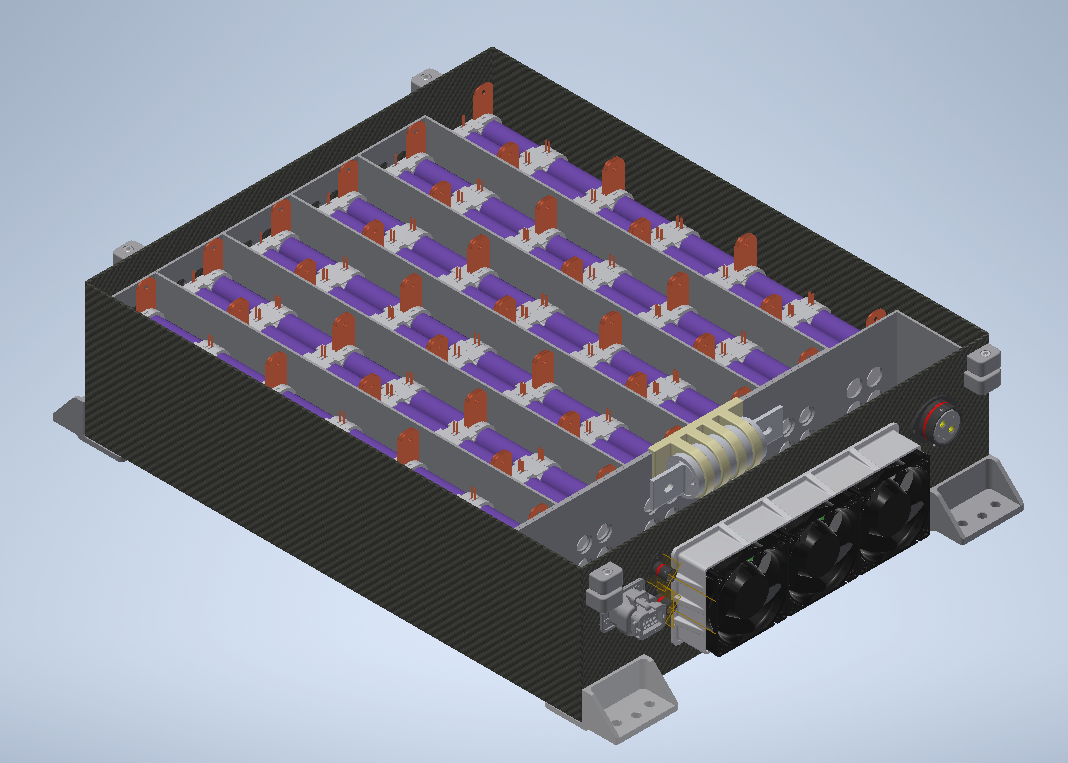
\includegraphics[scale=0.4]{pictures/pack.png}
    \caption{3D model of Fenice's battery pack}
    \label{fig:pack}
\end{figure}
The structure of a battery pack is decided considering its specific application. For example, in an high power context, higher voltage batteries are more desirable because for the same power draw, less current is required, decreasing heat losses across conductors. In high current applications, more cells in parallel could be arranged, increasing the total energy storage and battery weight as a consequence.

As mentioned above, a Formula SAE car's battery should be sized to complete a 22km endurance course while also being able to output the maximum amount of power for the acceleration event. The battery should also be optimized for weight and have a low center of gravity. Furthermore, the rulebook limits maximum voltage to 600V \cite[EV 4.1.1]{fsg2020} and power to 80kW \cite[EV 2.2.1]{fsg2020}, so the resulting battery will have as many cells in series as permitted and as few parallels as needed to reach the required power and capacity target.\\
Fenice's battery features 108 cells in series and 4 in parallel (108s4p), for a total of 432 cells and a nominal voltage of 388.8V. Higher voltages could be reached by rewiring the pack in a 144s3p configuration, but the pack would have a maximum voltage of 604.8V, exceeding the 600V limit. Adding more cells leads to increased weight, volume and excess of capacity.
The high power requirement of the pack is fullfilled by the use of high-discharge rate cells, amounting to 45A in Fenice's case. This results in a total output of 180A of continuous discharge current. As a consequence, The maximum theoretical power output of the whole pack approaches 70kW and the energy capacity amounts to 6.2kWh.

\subsubsection{Naming hierarchy}

\begin{figure}[h]
    \centering
    \begin{circuitikz}
    % Cell
    \draw (0,2) to[battery1] (0,3);
    \draw node[circle,draw,anchor=center,scale=4,label=Cell] (cell) at (0,2.5) {};

    % Cell to Module
    \draw node[circle,draw,anchor=center,scale=2.5] (ctm) at(2.25,2.5) {};
    \draw[->] (cell.east) -- (ctm.west);

    % Module
    \draw (2.75,1.5) -- ++(0,0.5) -| ++(-0.5,0) to[battery1] ++(0,1) -| ++(0.5,0.5)
    (2.75,2) -- ++(0.5,0) to[battery1] ++(0,1) -- ++(-0.5,0);
    \draw (3.25,2) edge[dotted] ++(0.5,0)
    (3.25,3) edge[dotted] ++(0.5,0);
    \draw node[circle,draw,anchor=center,scale=7,label=Module] (module) at (2.75,2.5) {};

    % Module to Block
    \draw node[circle,draw,anchor=center,scale=2.5] (mtb) at(6.5,2.5) {};
    \draw[->] (module.east) -- (mtb.west);

    % Block
    \draw (6.5,1) to[battery1] ++(0,1) to[battery1] ++(0,1) to[battery1] ++(0,1);
    \draw node[circle,draw,anchor=center,scale=9,label=Block] (block) at (6.5,2.5) {};

    % Block to Segment
    \draw[->] (block.east) -- (9.65,2.5);

    % Segment
    \draw (9.625,3) -- ++(0,+0.25);
    % 1
    \draw[solid] (9.5,2) rectangle ++(0.25,1);
    \draw (9.625,2) -- ++(0,-0.25) -| ++(0.5,0.25) ;
    % 2
    \draw[solid] (10,2) rectangle ++(0.25,1);
    \draw (10.125,3) -- ++(0,0.25) -| ++(0.5,-0.25) ;
    % 3
    \draw[solid] (10.5,2) rectangle ++(0.25,1);
    \draw (10.625,2) -- ++(0,-0.25) -| ++(0.5,0.25) ;
    % 4
    \draw[solid] (11,2) rectangle ++(0.25,1);
    \draw (11.125,3) -- ++(0,0.25) -| ++(0.5,-0.25) ;
    % 5
    \draw[solid] (11.5,2) rectangle ++(0.25,1);
    \draw (11.625,2) -- ++(0,-0.25) -| ++(0.5,0.25) ;
    % 6
    \draw[solid] (12,2) rectangle ++(0.25,1);
    \draw (12.125,3) -- ++(0,0.25);

    \draw node[circle,draw,anchor=center,scale=10,label=Segment] (segment) at (10.825,2.5) {};

    % Segment to Pack
    \draw[->] (segment.east) -- (14.15,2.5);

    % Pack
    \draw (14.125,3) -- ++(0,+0.25);
    % 1
    \draw[solid] (14,2) rectangle ++(0.25,1);
    \draw (14.125,2) -- ++(0,-0.25) -| ++(0.5,0.25) ;
    % 2
    \draw[solid] (14.5,2) rectangle ++(0.25,1);
    \draw (14.625,3) -- ++(0,0.25) -| ++(0.5,-0.25) ;
    % 3
    \draw[solid] (15,2) rectangle ++(0.25,1);
    \draw (15.125,2) -- ++(0,-0.25) -| ++(0.5,0.25) ;
    % 4
    \draw[solid] (15.5,2) rectangle ++(0.25,1);
    \draw (15.625,3) -- ++(0,0.25) -| ++(0.5,-0.25) ;
    % 5
    \draw[solid] (16,2) rectangle ++(0.25,1);
    \draw (16.125,2) -- ++(0,-0.25) -| ++(0.5,0.25) ;
    % 6
    \draw[solid] (16.5,2) rectangle ++(0.25,1);
    \draw (16.625,3) -- ++(0,0.25);

    \draw node[circle,draw,anchor=center,scale=10,label=Pack] (pack) at (15.4,2.5) {};

\end{circuitikz}
    \caption{Battery pack elements naming scheme}
    \label{fig:naming}
\end{figure}
As explained in figure \ref{fig:naming}, the pack is subdivided in physical blocks that can be summarised as follows:

\begin{itemize}
    \item The \textbf{cell} is the basic unit of the pack.
    \item Four cells in parallel form a \textbf{module} (also called cell, since the voltage is the same as a single cell).
    \item \textbf{Blocks} are a series of three modules, held together to form an actual block.
    \item The rulebook requires the separation of the pack into \textbf{segments} with precise physical and electrical characteristics \cite[EV 5.3.2]{fsg2020}. In this case a segment is a series of six blocks, totaling a maximum voltage of 75.6V ($4.2V*3\ modules*6\ blocks$) and 1.2kWh of energy, below the limit of 120V and 1.6 kWh mandated by the rules.
    \item In conclusion, the whole \textbf{pack} is composed of six segments connected in series.
\end{itemize}

\subsection{Internal Connections}
To be able to safely shut off the output of the battery pack, two normally-open Accumulator Isolation Relays (AIR) \cite[EV 5.6]{fsg2020} are located at both poles of the pack and are able to disconnect the battery from the outside of the battery container. These relays are controlled by the BMS and can also be switched off by external devices such as emergency buttons and sensors located around the car. In case of short-circuits, a fuse is also present between the negative contact and the input of the negative AIR.
\begin{figure}[h]
    \centering
    \ctikzset{bipoles/crossing/size=.6}
\begin{circuitikz} \draw
    (0,1) to[battery=\(BAT\),american] ++(0,3)

    %% Negative battery bus
    (0,4) to[fuse=\(F\)] ++(1.5,0) to[nos=\(AIR-\), n=airm] ++(2,0) -- ++(1.5,0)
    -- (5, 2.6) to[short, -*] ++(2,0) -- (7, 4.5) -- ++(1.5,0)

    %% Inverter 1
    (7, 2.4) to[short, *-] (7.75,2.4) -- (7.75,3.5) -- (8.5,3.5)
    (8.5,3.5) to[C=\(C_1\), n=c1, *-*] (8.5,4.5)

    (8.5,0.5) -- ++(0.75,0)
    (8.5,1.5) -- ++(0.75,0);
    \draw[solid] (9.25,3.25) rectangle ++(0.5,1.5);
    \path (9.25,3.25) -- ++(0,-0.5);
    \draw[dotted] (7.3,5) rectangle (10,3) node[at start, right, fill=white] {Inverter 1};

    %% Positive battery bus
    \draw (0,1) to[nos=\(AIR+\), n=airp] ++(5,0)
    to (5,2.4) -- ++(2,0) -- (7, 0.5) -- ++(1.5,0)

    %% Inverter 2
    (7, 2.6) to[crossing] ++(1.5,0) -- (8.5,1.5)
    (8.5,0.5) to[C=\(C_2\), *-*] (8.5,1.5)

    (8.5,3.5) -- ++(0.75,0)
    (8.5,4.5) -- ++(0.75,0);
    \draw[solid] (9.25,1.75) rectangle ++(0.5,-1.5);
    \draw[dotted] (7.3,0) rectangle (10,2) node[at start, right, fill=white] {Inverter 2};

    %% Pre-charge circuit
    \draw (0.5,1) to[short, *-] ++(0,-1)
    to[nos=\(S_p\),n=pre_sw] ++(2, 0)
    to[R=\(R_p\),n=pre_sw] ++(2,0)
    to[short, -*] ++(0,+1)

    {[anchor=north] (6,2.4) node {\(Bus_+\)} [anchor=south] (6,2.6) node {\(Bus_-\)}};

    %% Motor 1
    \draw (11,4) node[elmech](M1){M1}
    (9.75,4.65) -- ++(0.75,0) -- (M1.150)
    (9.75,4) -| (M1.180)
    (9.75,3.35) -- ++(0.75,0) -- (M1.210)
    ;

    %% Motor 2
    \draw (11,1) node[elmech](M2){M2}
    (9.75,1.65) -- ++(0.75,0) -/ (M2.150)
    (9.75,1) -| (M2.180)
    (9.75,0.35) -- ++(0.75,0) -/ (M2.210)
    ;

    \draw[dotted] (-2,5) rectangle (5.25,-0.5) node[at start, right, fill=white] {Battery Pack};


\end{circuitikz}
    \caption{Tractive system schema}
    \label{fig:tractive_system_detail}
\end{figure}
\subsubsection{Precharge}
If the power-on procedure of the pack simply involved putting both AIRs to their closed position, a potentially dangerous in-rush current would charge the capacitors on the inverters very quickly. To control prevent overcurrent, the precharge procedure is performed.
First, the negative AIR together with $S_p$ is closed. This operation creates an alternative circuit that has $R_p$ as the current-limiting resistor. After $Bus$ and $BAT$ voltages have equalized, the positive AIR can finally be closed. This completes the precharge procedure and the battery is ready to be used.

\subsection{Battery Management Hardware}
The need to measure a large amount of voltages and temperatures scattered around the battery pack leads to a decentralized structure for the BMS components. Two types of logic boards are involved, namely the \textbf{Mainboard} and the \textbf{Cellboard}.\\
\begin{figure}[h]
    \centering
    
\begin{tikzpicture}[
        text=blue,
        carnode/.style={inner sep=-11pt},
        mainnode/.style={rectangle, draw=red, fill=red!15, very thick, minimum size=10mm},
        cellnode/.style={rectangle, draw=yellow, fill=yellow!15, very thick},
        arrow/.style={<->, >=stealth, fill=white, draw=blue, very thick}
    ]


    %Nodes
    \node[carnode]  (car)                       {
\includegraphics[width=0.3\textwidth, page=1]{silhouette.pdf}};
    \node[mainnode] (main)  [right=2cm of car]  {Mainboard};
    \node[cellnode] (c3)    [right=of main]     {Cellboard 3};
    \node[cellnode] (c2)    [right=of c3]       {Cellboard 2};
    \node[cellnode] (c1)    [above=of c2]       {Cellboard 1};
    \node[cellnode] (c0)    [left=of c1]        {Cellboard 0};
    \node[cellnode] (c4)    [below=of c3]       {Cellboard 4};
    \node[cellnode] (c5)    [right=of c4]       {Cellboard 5};

    %Lines
    \path [arrow] (main.north) node[anchor=south east] {\scriptsize{$master$}} |- node[above, fill=white] {CAN-bus} (c0.west);
    \path [arrow] (car.south) |- ++(0,-1) -- ++(2,0) node[fill=white] {CAN-bus} -| (main.south);

    \draw[arrow] (c0.east) -- (c1.west);
    \draw[arrow] (c1.south) -- (c2.north);
    \draw[arrow] (c2.west) -- (c3.east);
    \draw[arrow] (c3.south) -- (c4.north);
    \draw[arrow] (c4.east) -- (c5.west);

    %\draw let \p1=(main) \p2=(c0) in node at (\x1,\y2) {k};
    \draw[thick,dotted] ($(main.north west)+(-0.5, 2)$) rectangle ($(c5.south east)+(0.5, -0.5)$) node[at start, right, fill=white] {Battery};

\end{tikzpicture}

    \caption{BMS hierarchy}
    \label{fig:bms_hierarchy}
\end{figure}

\subsubsection{Mainboard}
%\begin{figure}[h]
%    \centering
%    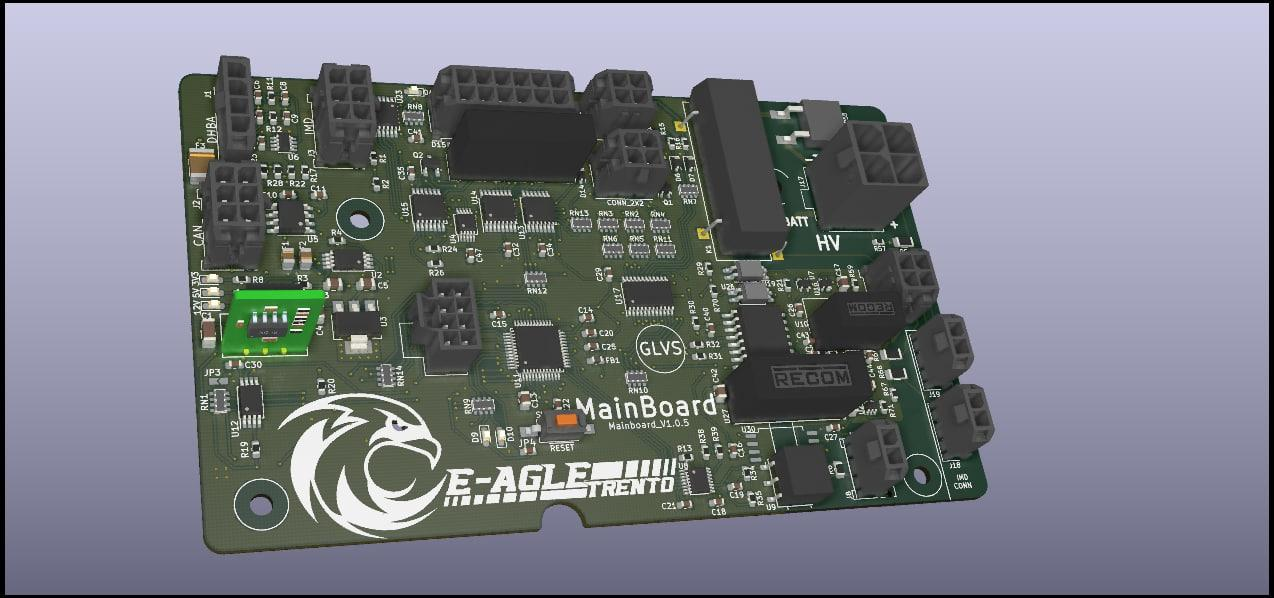
\includegraphics[scale=0.5]{pictures/mainboard.jpg}
%    \caption{Mainboard PCB}
%    \label{fig:mainboard}
%\end{figure}
The Mainboard is the central control unit of the BMS. It consists of a microcontroller that handles the pre-charge circuit, two CAN-bus lines and peripherals such as ADCs, EEPROMs and more. The mainboard is responsible for the actuation of the AIRs and contains the precharge circuit. It also handles communication with the rest of the car about the battery status, warnings and errors.

\subsubsection{Cellboard}
There are a total of six cellboards on Fenice's battery pack, one for every battery segment. Cellbaords are dedicated to the measurement of module voltages and cell temperatures. The reading of voltages is handled by a specialized battery management chip that communicates via SPI to the on-board microcontroller. Temperatures are acquired with sensors glued to the cells. All the data collected from the boards is sent via an internal CAN-bus to the mainboard.\
Cellboards are also in control of cell balancing. They can activate and deactivate discharging for any module through the battery management chip, depending on commands from the mainboard.

\section{Issues}
\subsection{Battery Management}
Battery management is a collection of operations that ensure the safety and efficiency of the battery pack's functioning.\\
A battery management system should constantly measure cell temperatures and voltages along with the total pack current output and check that each of those values is within specification. If anomalies are detected, the battery should be disconnected immediately.\\
Advanced BMS implementations communicate their state of operation with other devices, and turn the battery on or off according to external signals.\\
Moreover, during battery charging, the BMS should handle the charge current curve to maximize charging speed while keeping the battery in a safe state.\\
As the consequences of software errors on the BMS are potentially catastrophic, the code must adhere to strict standards and should be tested thoroughly. Furthermore, a reliable error management should be present to abide to the rulebook and to ease troubleshooting.

\subsection{Module Balancing}
Cells are not perfectly identical and can have slight variations in internal resistance between each other. These differences mean that after some use, modules can start to deviate in voltage between one another. If a cell has an higher voltage than average, the pack can only be charged to the voltage of said cell, while the remaining modules don't get fully charged. The same applies during discharge: if a module is more discharged than others, it constraints the maximum depth of discharge to when it reaches its cutoff voltage, while other cells are still above it and could theoretically be discharged further.\\
This issue limits the maximum energy storage available for use, reducing the car's range.

